\begin{comment}

TODO: Data exploration
TODO: Data pre-processing
TODO: Dealing with missing data
TODO: Moving average smoothing
TODO: Results

\end{comment}

An essential step between acquiring of the data and passing it to machine learning algorithms is ensuring that the dataset used for training represents our learning objectives. In this case, our learning objective is to train the system to recognize two of the well-known gymnastics movements - the backflip and the back handspring. A well-balanced and interpretable dataset is necessary for avoiding overfitting or biasing the machine learning model to a specific dataset. 

In section \ref{data-exploration}, we start by sampling the data and visualizing it to better understand the pose estimation results obtained in the previous chapter. Then, based on the observations, pre-processing strategies for overcoming the shortcomings of the dataset are proposed by the author in section \ref{data-pre-processing-strategies} and lastly the final dataset, ready to be used for machine learning, is described in the \ref{pre-processing-results} section of this chapter.

\section{Data exploration}
\label{data-exploration}

During the data acquisition phase, individual csv files (figure \ref{sample-body-parts-by-openpose}) were generated for each frame of each sample recording. Since the data is generated for each frame, one suitable visualization method is the time-series line plot. Each frame's data contains 25 estimated keypoints, both \textit{X} and \textit{Y} coordinates for each keypoint and also the Confidence Score issued by OpenPose. Given the amount of dimensions for such dataset, a sample entity with the following parameters is chosen for demonstration purposes:

\begin{easylist}[itemize]

& \textit{Sample activity} --- Back handspring
& \textit{Sample no.} --- 17
& \textit{Keypoint index} --- 21 (left heel), figure \ref{pose-output-format}
& \textit{Axis} --- Y

\end{easylist}

There is no particular reason for choosing the left heel of the subject, other than given the rotation of the subject's body during the sample activity, we can expect the data range of the left heel's position to vastly differ on the \textit{Y} axis. This is because the subject's body will be upside down at some point during the movement.

The figure \ref{lack-17-rasmus-l-heel-y-raw} represents the subject's left heel's trajectory along the \textit{Y} axis during the back handspring. For the first second of the activity, the pose estimation seems to not have problems recognizing the left heel during the momentum generation phase. For the takeoff, rotation and landing phase the pose estimation's confidence score falls under the threshold and results in filling the low confidence frames with the zero values. This makes the data not usable by machine learning algorithms, since such strong deviations can be labeled as anomalies and will most likely strongly affect the gradient computed during the backpropagation, ultimately making the algorithms learn something else besides the activities investigated.

\begin{figure}[htb]
  \centering
    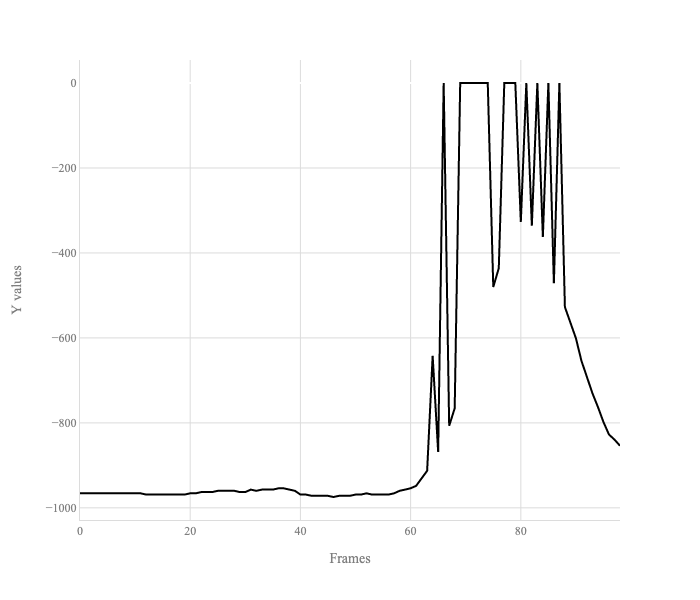
\includegraphics[width=\textwidth,keepaspectratio]
    {images/data-preprocessing/flack-17-rasmus-l-heel-y-raw}
    \caption{Subject's left heel trajectory during the back handspring - raw data}
    \label{lack-17-rasmus-l-heel-y-raw}
\end{figure}

\section{Data pre-processing\\strategies}
\label{data-pre-processing-strategies}

Four mitigation steps are chosen to overcome the shortcomings of initial pose estimation results. It is worth mentioning, that for clear interpretation purposes the strategies described in next sections are demonstrated on a single sample. Python scripts were developed by the author to automatically apply all pre-processing strategies on every sample's every body part for all frames.

\subsection{Dealing with low confidence keypoints}

During the pose estimation process described in Chapter \ref{data-acquisition}, a confidence score in the range of 0-1 is issued for each keypoint by OpenPose. The confidence score represents OpenPose's certainty when determining keypoints of the subject. Confidence score of 0 by OpenPose means the system fails to estimate a particular body part in a frame. For a keypoint with confidence score approaching 1, translates to a high confidence in detecting the specific keypoint. 

A simple algorithm was implemented by the author to fill the missing keypoints - moving through frames and filling missing keypoints with the averages of existing keypoint with positive confidence score, figure \ref{moving-average-filling-algorithm}. The improved sample's subject left heel trajectory can been seen on figure \ref{lack-17-rasmus-l-heel-y-filled}.

\begin{figure}[htb]
  \centering
    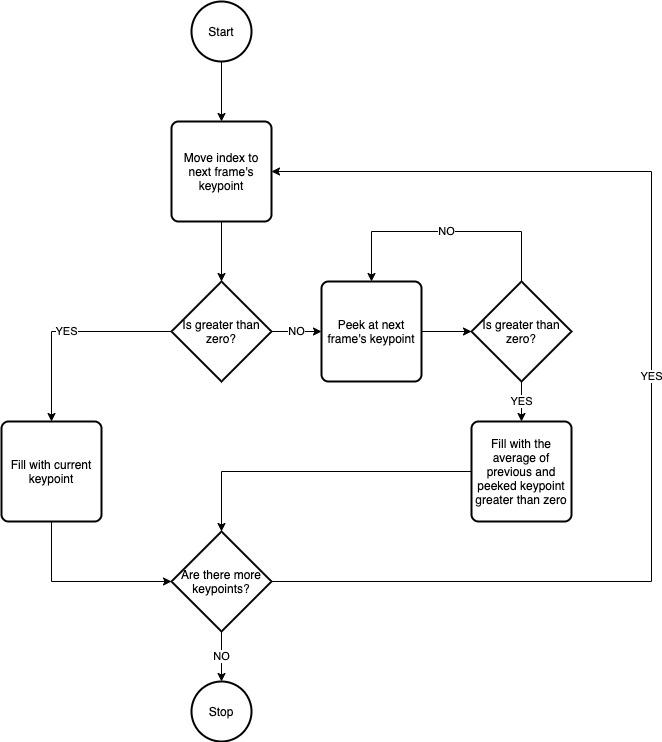
\includegraphics[width=0.7\textwidth,keepaspectratio]
    {images/data-preprocessing/moving-average-filling-algorithm}
    \caption{Moving average filling algorithm}
    \label{moving-average-filling-algorithm}
\end{figure}

\begin{figure}[htb]
  \centering
    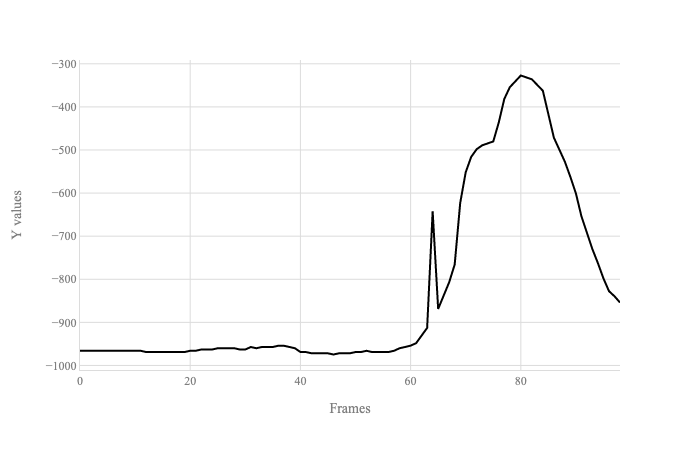
\includegraphics[width=\textwidth,keepaspectratio]
    {images/data-preprocessing/flack-17-rasmus-l-heel-y-filled}
    \caption{Subject's left heel trajectory during the back handspring - filled}
    \label{lack-17-rasmus-l-heel-y-filled}
\end{figure}

\subsection{Moving average smoothing}

During the pose estimation process described in section \ref{pose-estimation-process-and-results}, the OpenCV library is used to access each frame of the recordings. The frame's data is then fed into OpenPose's estimation function and estimated keypoints are obtained for each frame. The process is stateless by design, so nor previous or next estimations are taken into account when estimating the current frame. This results in fine-grained variations between frames. \textit{Moving Average Smoothing} is a technique applied to time series data in hope to remove noise and better expose the signal of the underlying process.

We define the moving average in the formula \ref{moving-average-smoothing-formula}. More specifically, the moving average formula defined can be categorized as the \textit{centered moving average}. We use the centered version of the moving average, since all values in the set are known prior to the smoothing phase. In the formula, we use \textit{n} of 3 and define it as the width of the moving window. The \textit{x} defined in the formula is the set of values for each body part coordinate for every frame of the activity. Figure \ref{lack-17-rasmus-l-heel-y-smoothed} displays the transformed left heel's trajectory after applying the smoothing technique.

\begin{equation}
\label{moving-average-smoothing-formula}
x(t) = \dfrac{1}{n}\sum\limits_{i=-\left\lfloor{\dfrac{n}{2}}\right\rfloor}^{\left\lfloor{\dfrac{n}{2}}\right\rfloor}x_{t+i}
\end{equation}

\begin{figure}[htb]
  \centering
    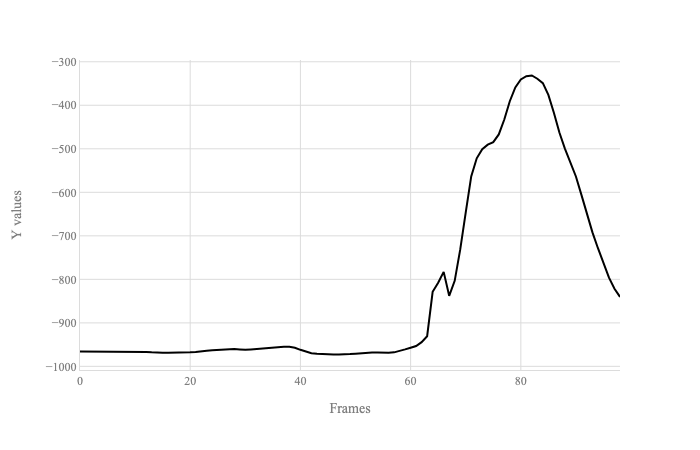
\includegraphics[width=\textwidth,keepaspectratio]
    {images/data-preprocessing/flack-17-rasmus-l-heel-y-smoothed}
    \caption{Subject's left heel trajectory during the back handspring - smoothed}
    \label{lack-17-rasmus-l-heel-y-smoothed}
\end{figure}

\subsection{Unrecognizable body parts}

One limitation worth mentioning when using the pose estimation technique is the contrast between the background and the athlete in the recordings. In low light and low contrast environments, the body parts of an athlete are not easily recognizable (as demonstrated in figure \ref{example-of-unrecognizable-backflip}), which leads to low confidence score for some body parts and makes it impossible to construct a full skeleton. Possible solutions (not explored in this thesis), to improve the recognition of body parts in low contrast environments, include controlling the contrast of the recordings with some post production software or rerecording the activities with athletes wearing clothes with a higher contrast against the background. For this thesis, however, the samples with unrecognizable body parts were left out of the dataset during the preprocessing phase.

\begin{figure*}
   \centering
\begin{tabular}{ccc}
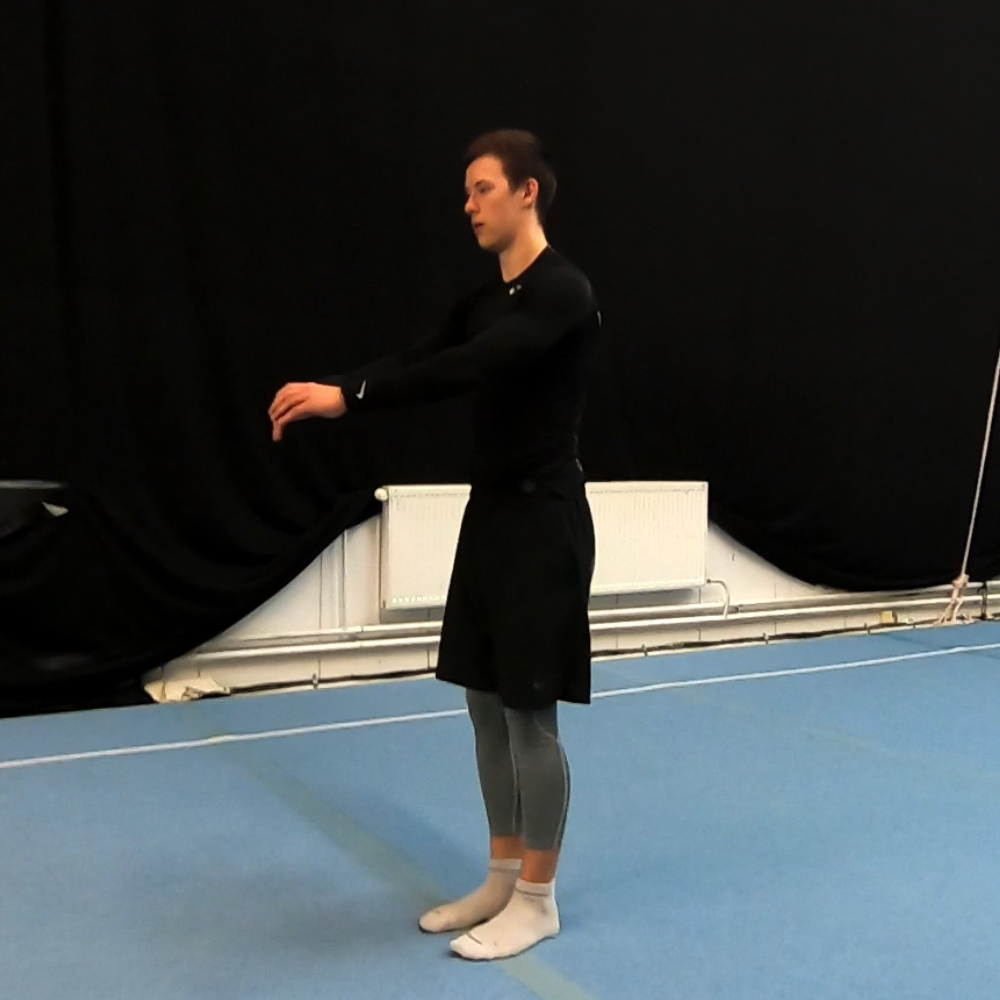
\includegraphics[width=5cm]{images/data-preprocessing/unrec-backflip-part-1}&
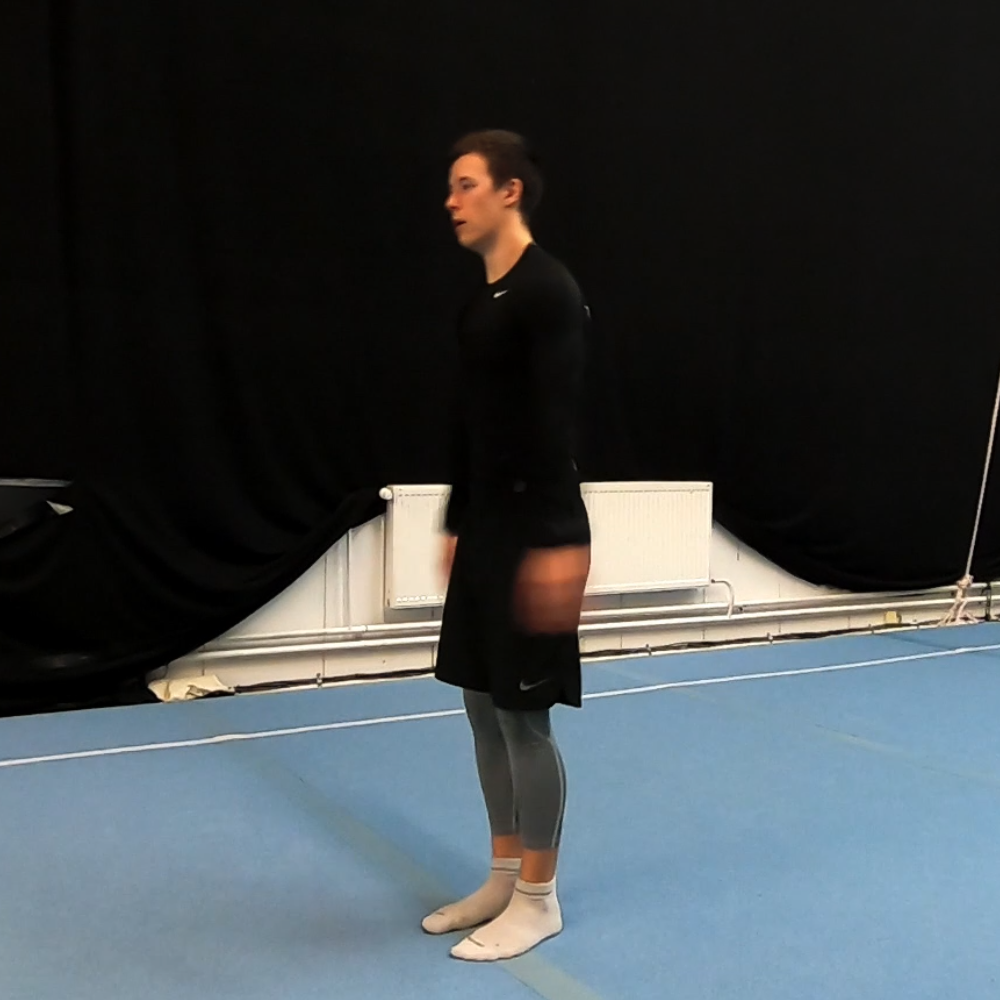
\includegraphics[width=5cm]{images/data-preprocessing/unrec-backflip-part-2}&
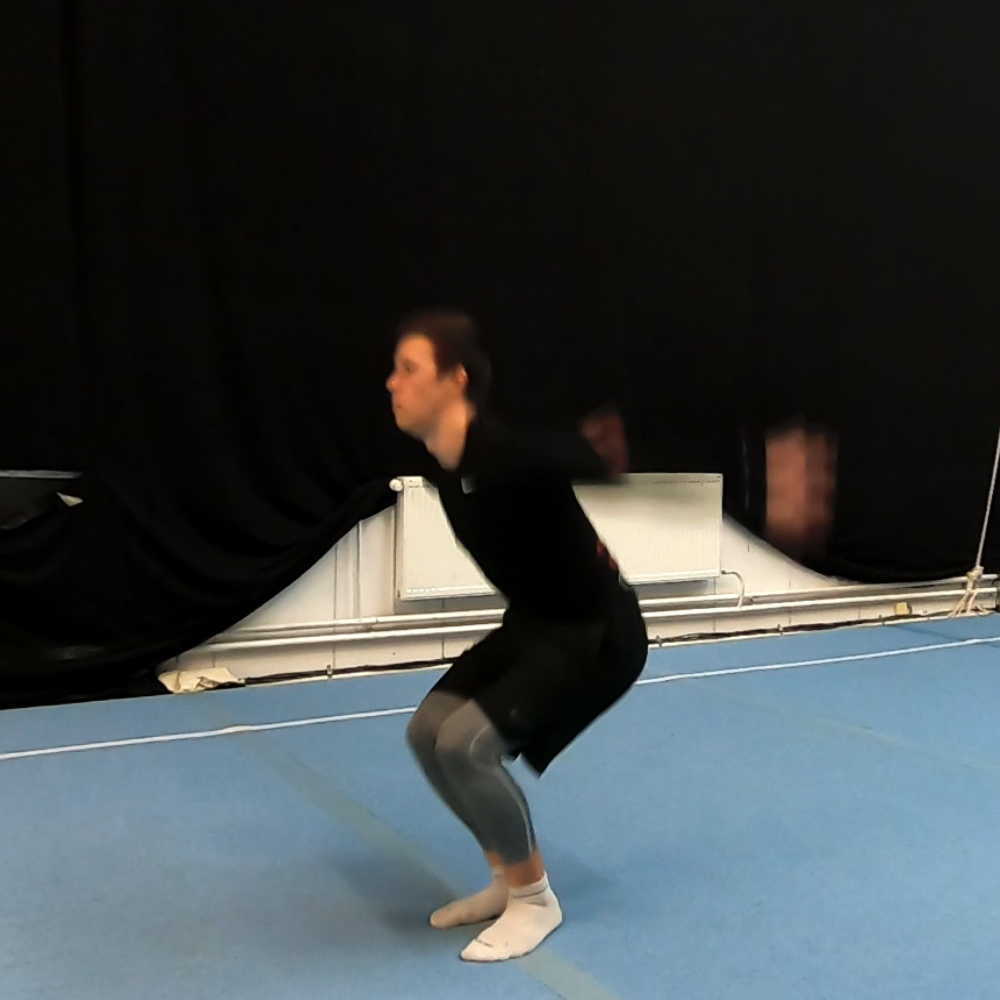
\includegraphics[width=5cm]{images/data-preprocessing/unrec-backflip-part-3}\\
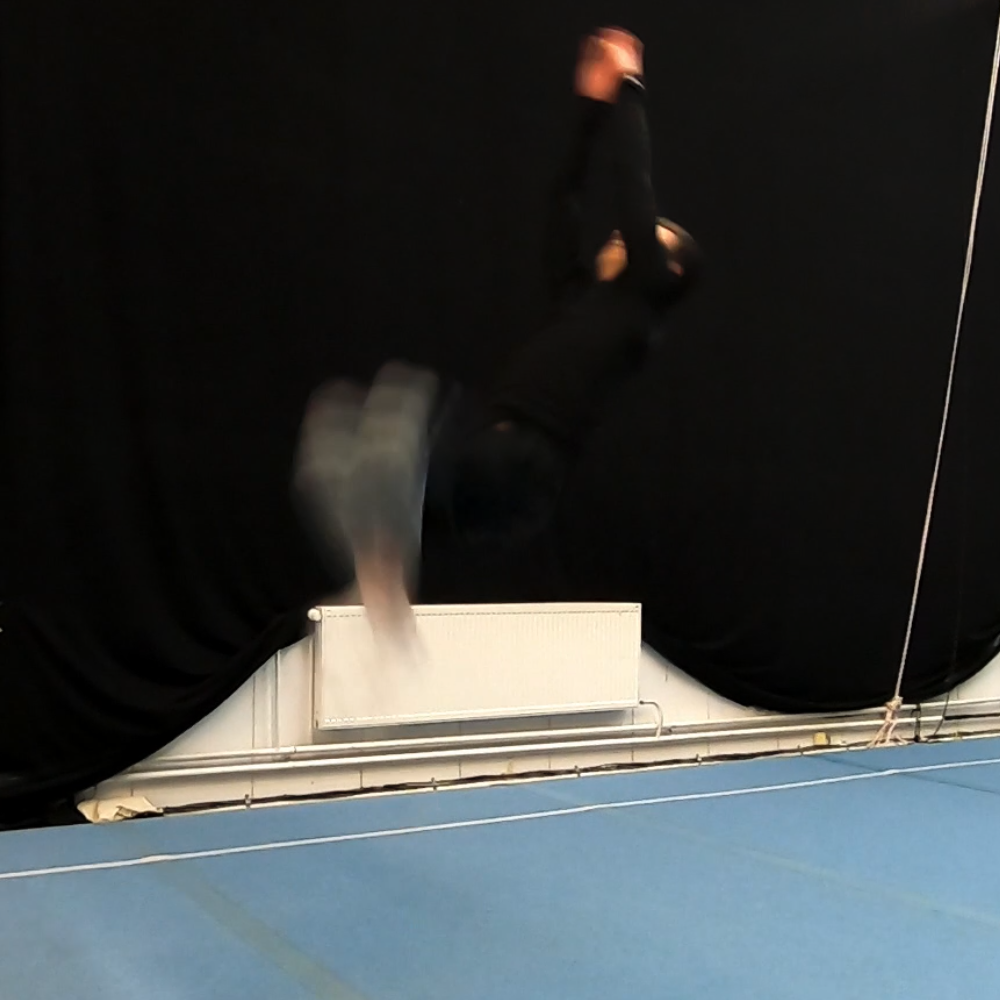
\includegraphics[width=5cm]{images/data-preprocessing/unrec-backflip-part-4}&
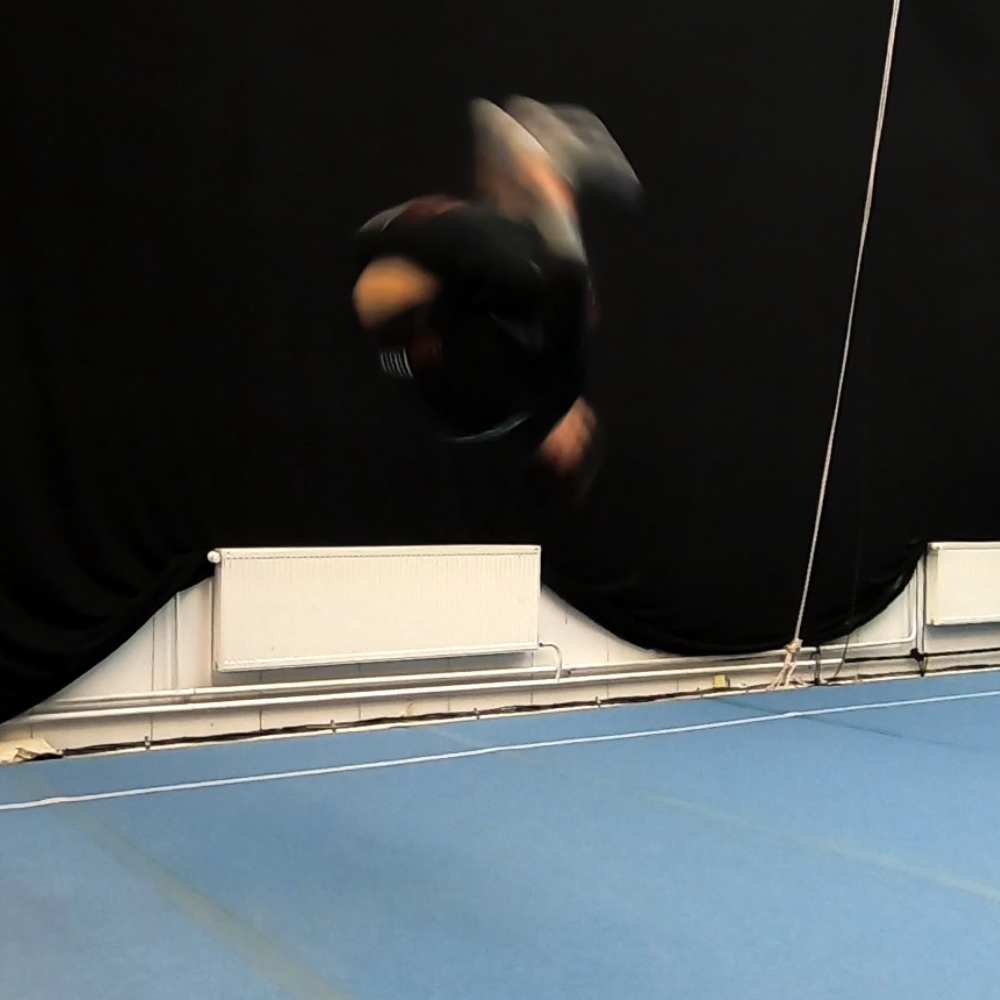
\includegraphics[width=5cm]{images/data-preprocessing/unrec-backflip-part-5}&
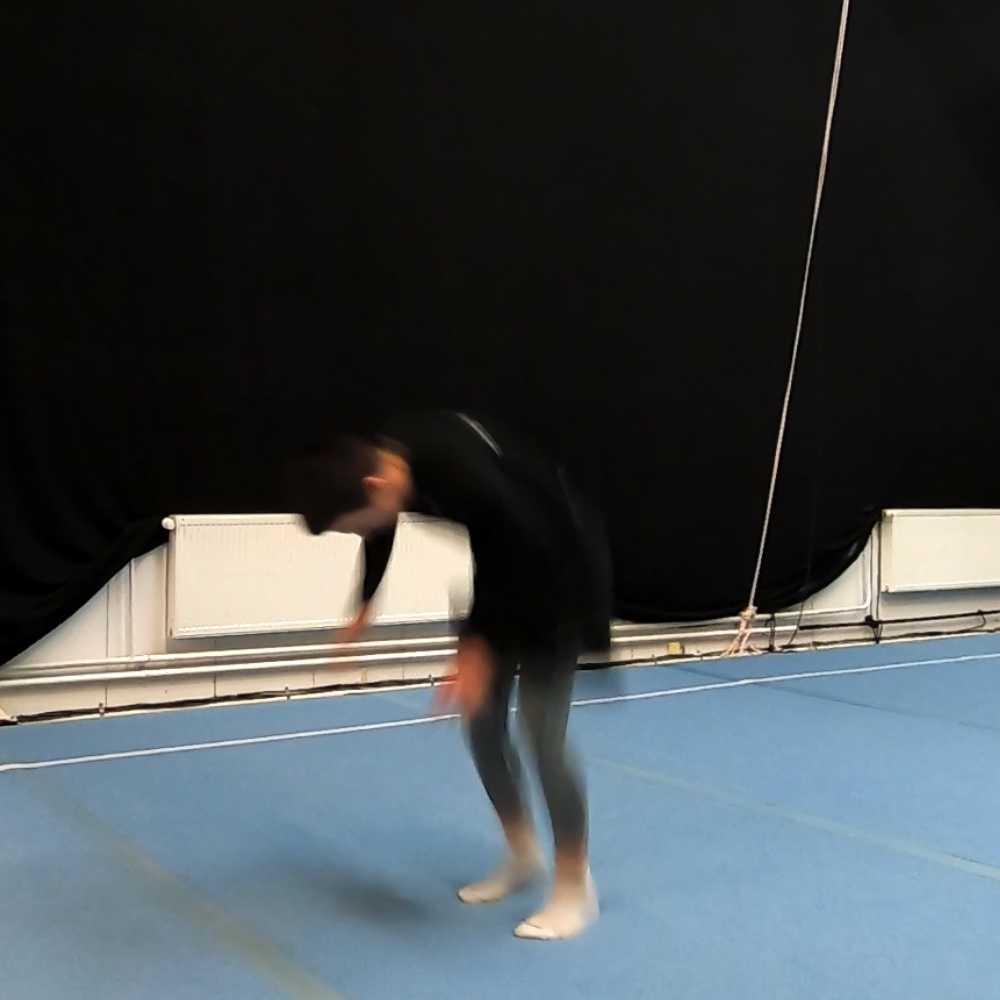
\includegraphics[width=5cm]{images/data-preprocessing/unrec-backflip-part-6}\\
\end{tabular}
    \caption{The movement of some body parts during this backflip sample are unrecognizable}
    \label{example-of-unrecognizable-backflip}
\end{figure*}

\subsection{Centering to unified coordinate origin}

Inspired by data pre-processing methods in \cite{hierarchical-rnn-har}, the authors Yong Du, Wei Wang and Liang Wang remarkably point out that human actions are independent of its absolute spatial position. Since the starting coordinates of gymnastics movements were not defined prior to recording the actions, normalizing the samples to a unified coordinate origin greatly decreases fluctuations between the same features. All samples in this paper are normalized to the coordinate system origin using the middle hip keypoint indexed as 8 in the \textit{BODY\_25} model. The figure \ref{centered-backflip-4-rasmus} demonstrates how the skeleton moves relative to the coordinate system origin after normalization.

\begin{figure*}
   \centering
\begin{tabular}{ccc}
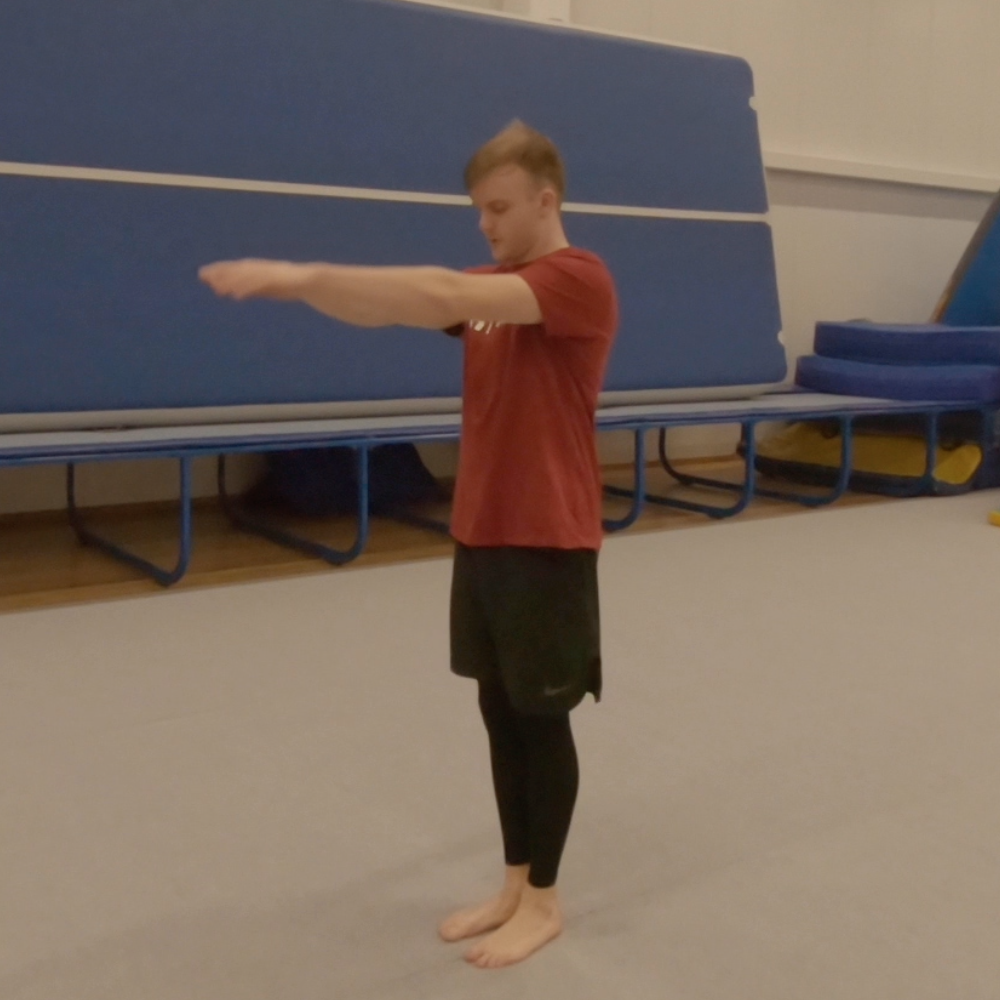
\includegraphics[width=5cm]{images/data-preprocessing/centered-backflip-orig-part-1}&
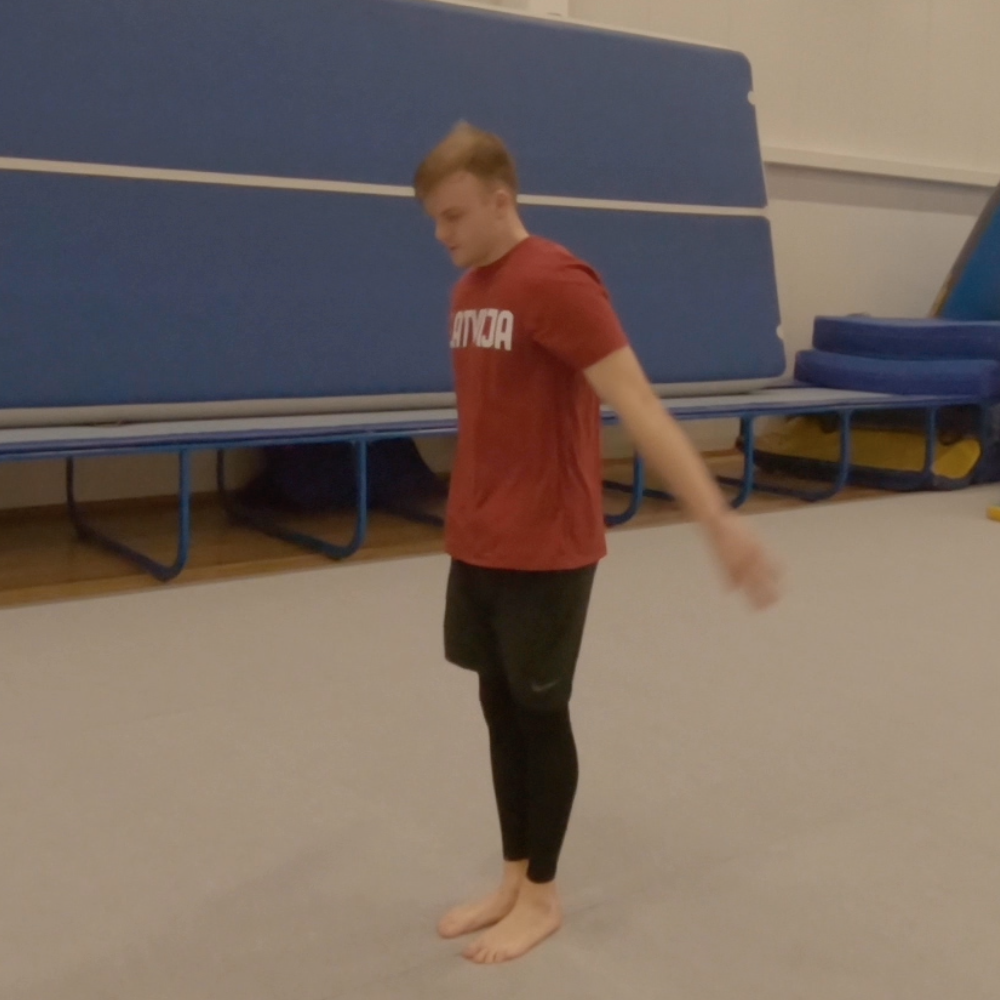
\includegraphics[width=5cm]{images/data-preprocessing/centered-backflip-orig-part-2}&
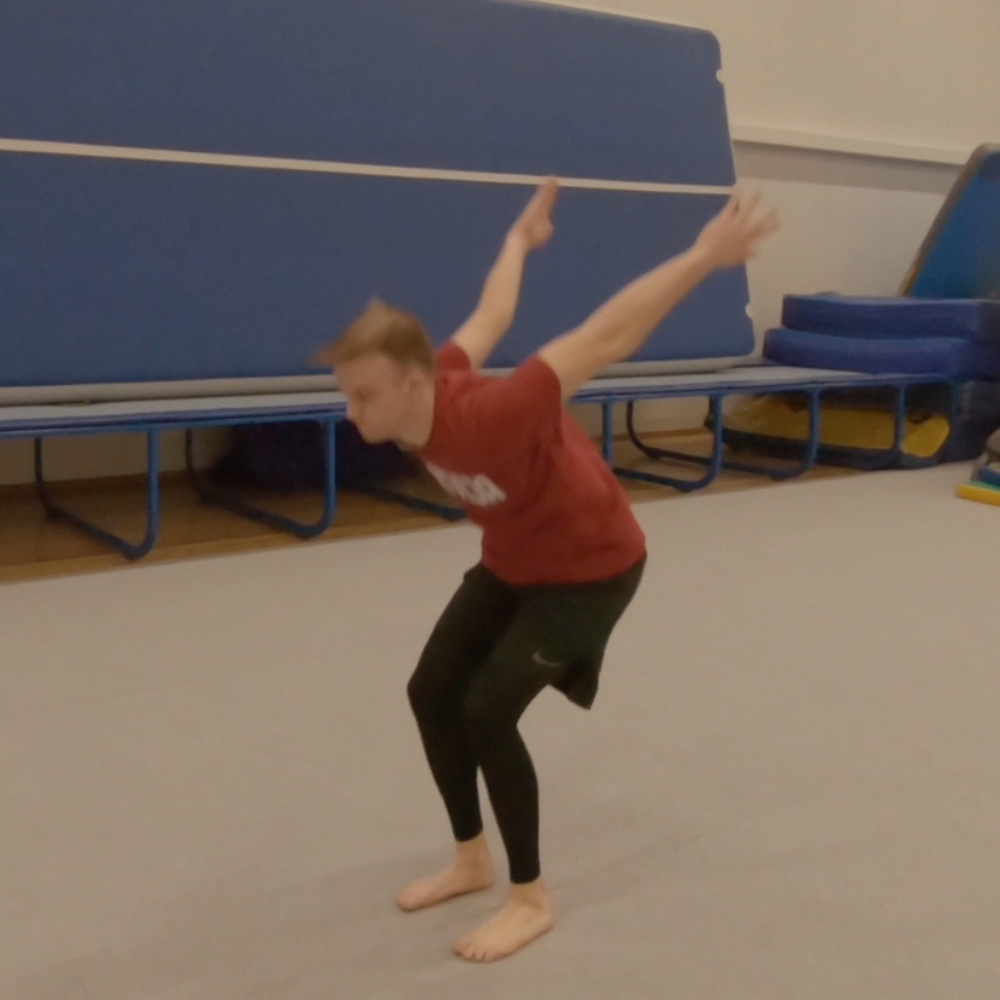
\includegraphics[width=5cm]{images/data-preprocessing/centered-backflip-orig-part-3}\\
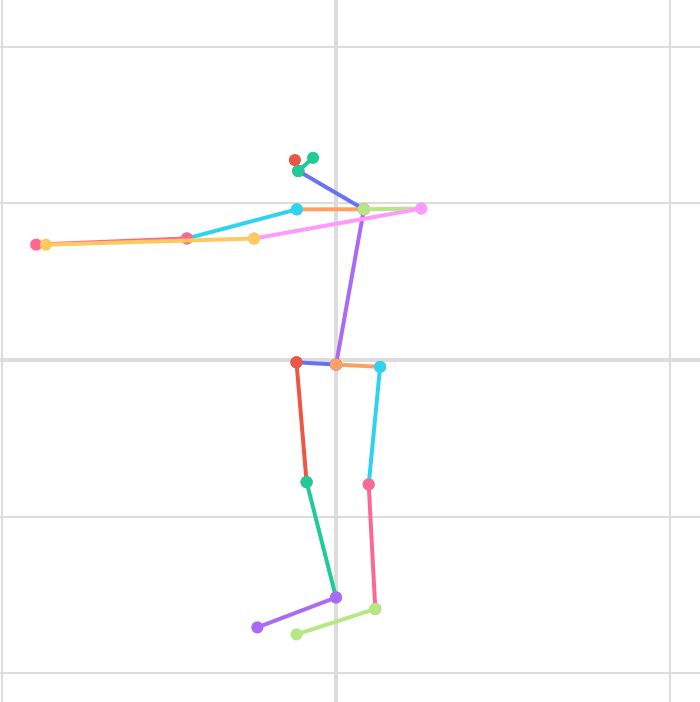
\includegraphics[width=5cm]{images/data-preprocessing/centered-backflip-skel-part-1}&
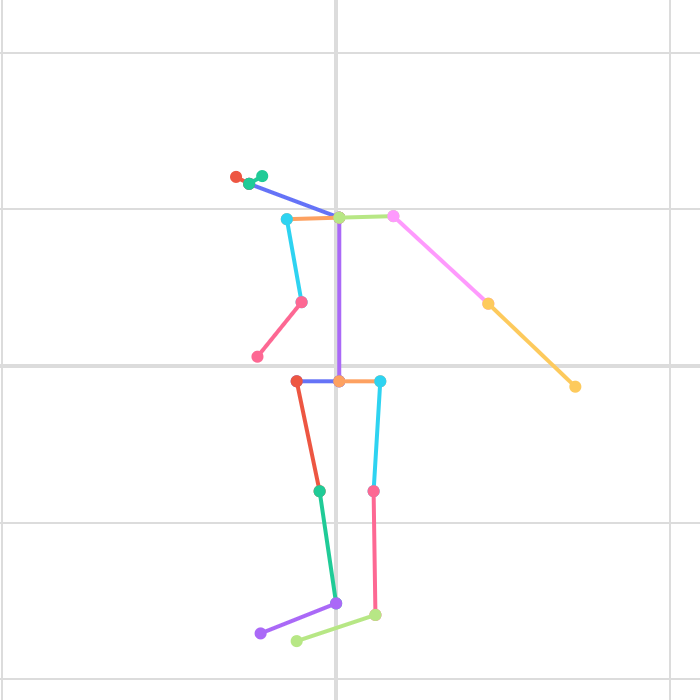
\includegraphics[width=5cm]{images/data-preprocessing/centered-backflip-skel-part-2}&
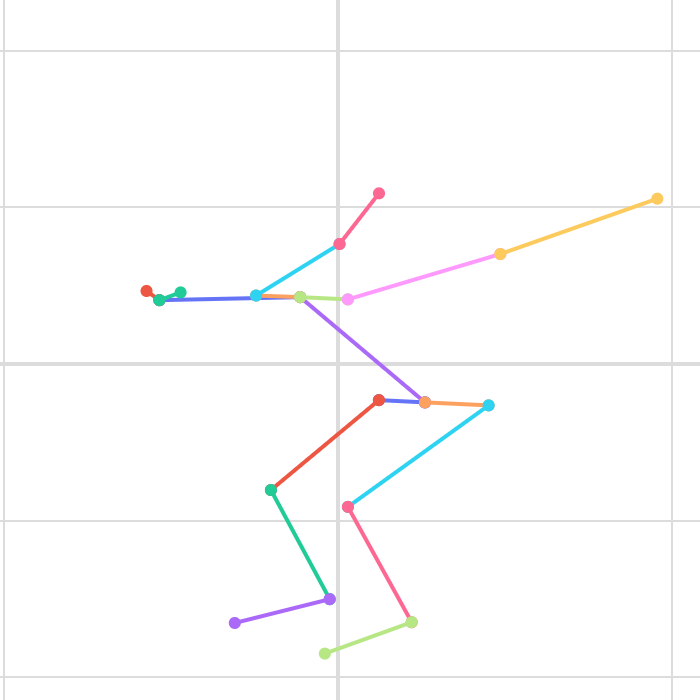
\includegraphics[width=5cm]{images/data-preprocessing/centered-backflip-skel-part-3}\\
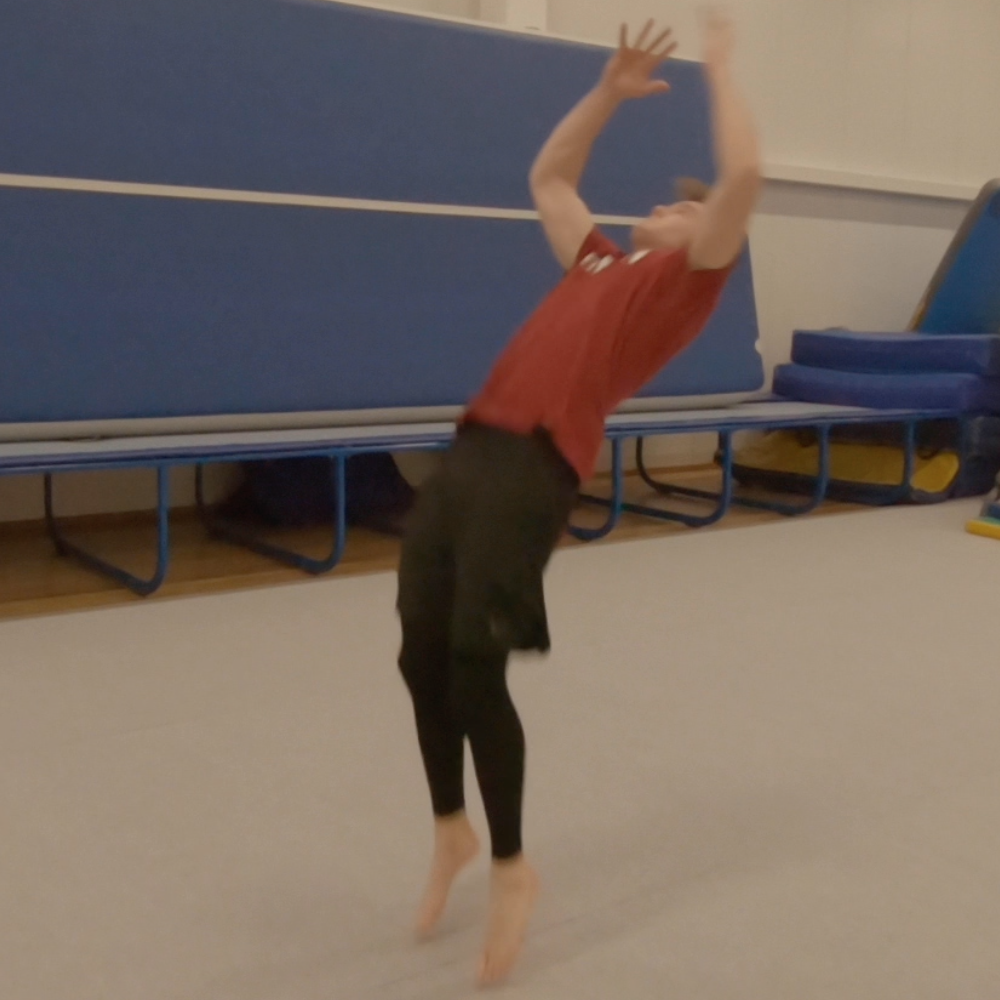
\includegraphics[width=5cm]{images/data-preprocessing/centered-backflip-orig-part-4}&
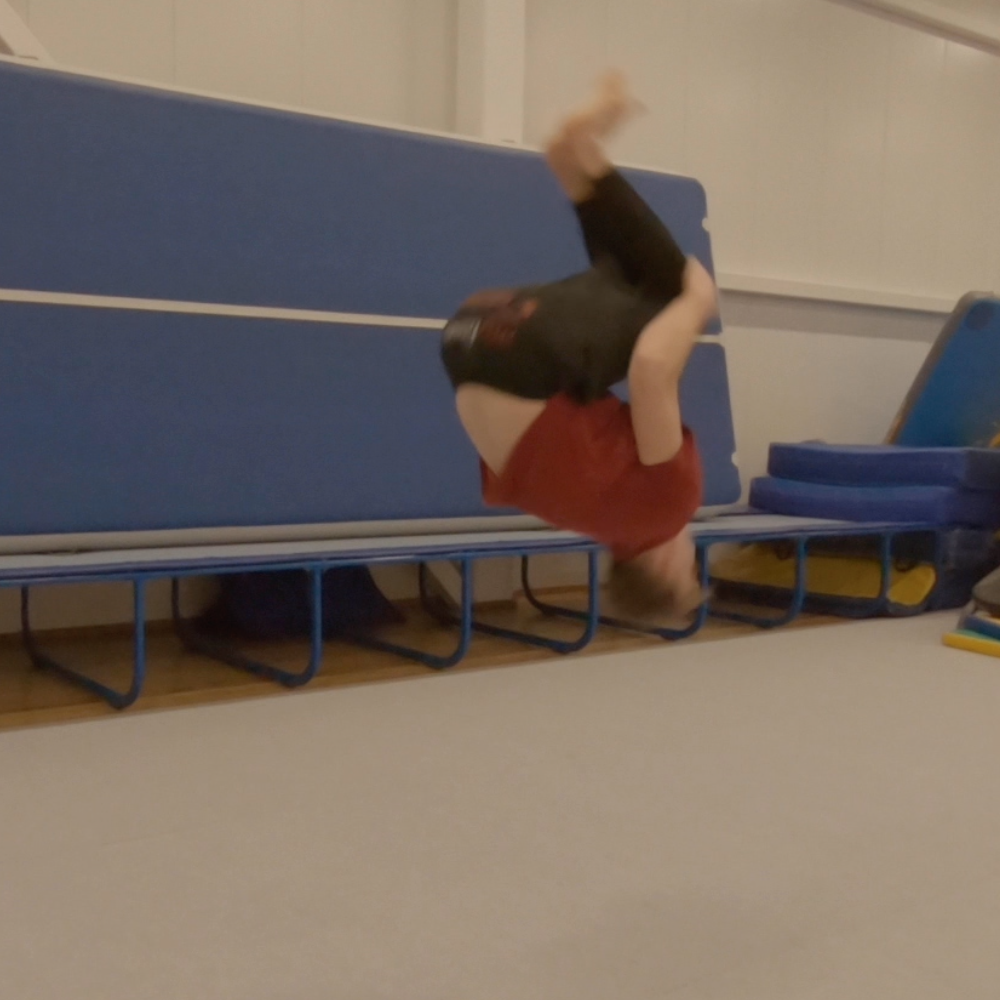
\includegraphics[width=5cm]{images/data-preprocessing/centered-backflip-orig-part-5}&
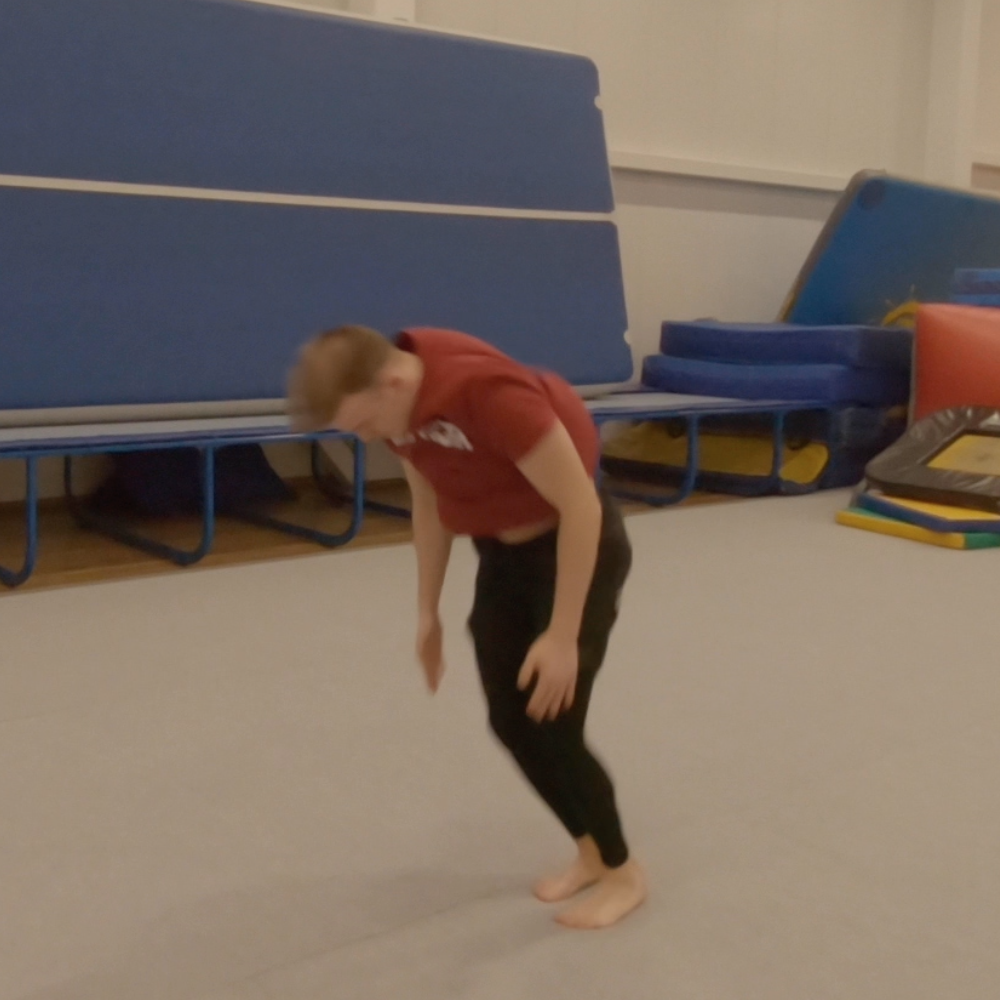
\includegraphics[width=5cm]{images/data-preprocessing/centered-backflip-orig-part-6}\\
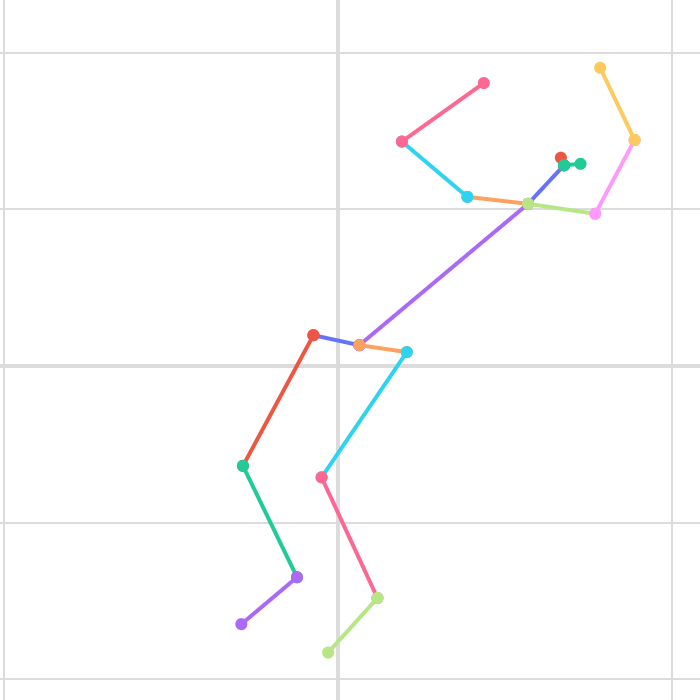
\includegraphics[width=5cm]{images/data-preprocessing/centered-backflip-skel-part-4}&
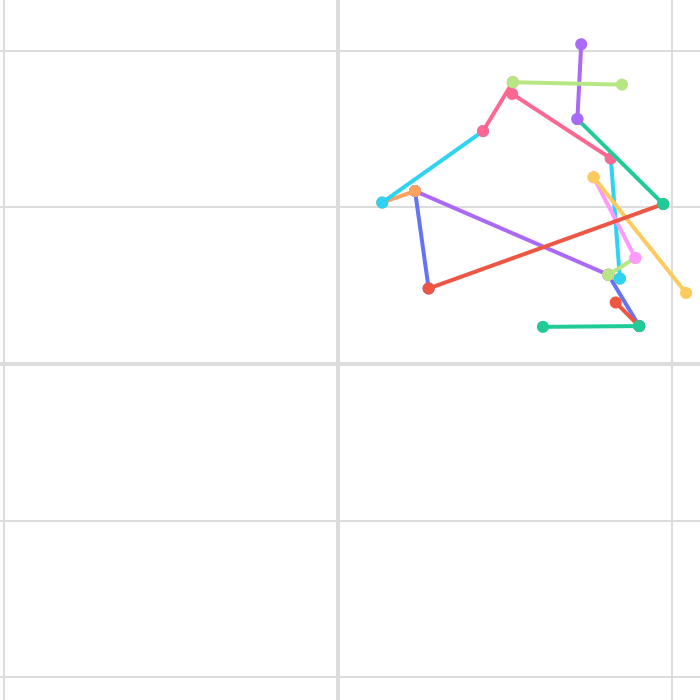
\includegraphics[width=5cm]{images/data-preprocessing/centered-backflip-skel-part-5}&
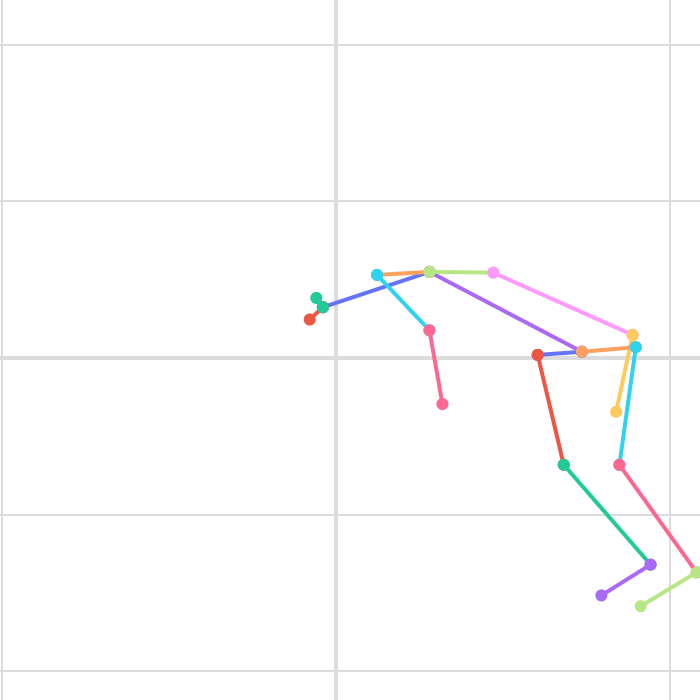
\includegraphics[width=5cm]{images/data-preprocessing/centered-backflip-skel-part-6}\\
\end{tabular}
    \caption{Backflip sample centered to coordinate system origin}
    \label{centered-backflip-4-rasmus}
\end{figure*}

\subsection{Data augmentation}

To train classifiers and validate for generalization, one is required to supply well-balanced and a greater amount of data in order to avoid overfitting neural network models to specific samples. The result of 113 samples obtained through previous data processing strategies is enough for building network architectures, however the amount is not enough to validate the model for overfitting. There are many augmentation strategies applicable to skeleton manipulation \cite{NUNEZ201880}. 

The strategy chosen in this case applies random displacement degrees between local joints of the skeleton. Intuitively, pairs of directly connected keypoints are found, after which a pseudo-random degree between 0 and 15 is generated for each pair. Rotation is then applied for the pair of joints for every frame in the sample. Finally, this augmentation is repeated for 100 times, amplifying the previous 113 samples to a total of 11300 new augmented samples.

\section{Results}
\label{pre-processing-results}

The final dataset yielded after applying all pre-processing strategies consists of 5100 backflip and 6200 back handspring samples, totaling to 11300 samples. The samples are persisted as \textit{csv} files for each frame of each sample.

